\section{The Data Acquisition Toolkit}

%%%  An introduction of the idea of the "DAQ toolkit"
%%   mention Gen-I, Gen-II, Gen-III somewhere

%The New ROD Complex (NRC) is designed as a plug compatible replacement for the current complex. The interfaces necessary to satisfy that plug compatibility were described in Chapter 1. At one level of abstraction the physical implementation of the NRC could be simply represented as an arbitrary aggregate of PCB boards. But, of course, because these boards operate to a single purpose, they will also necessarily require connections between them. Typically, for reasons of understanding, modularity and maintenance, those connections follow predefined, accepted mechanical and electrical standards. In this document any such usage which employs a specific standard will be referenced as a Platform. For example, VME would constitute one such platform. For the NRC that platform is based on an existing standard developed by the PCI Industrial Computer Manufactures Group (PICMG) commonly referred to as the Advanced Tele-Communication Architecture, or ATCA, whose current revision is referred to within that consortium as PICMG 3.0. As a platform ATCA is now quite mature, having been in existence for more than ten years, with a broad design base and a wealth of equipment deployed in the field as well as a burgeoning eco-structure within the telecommunication and defence industries.
%ATCA usage by the NRC will be entirely compliant with the PICMG 3.0 specification. That specification is described in [6] with an introduction available from [5]. However, the remainder of this section is intended to provide sufficient background to gain a thorough understanding of the physical design description.

In this section we give a brief introduction the DAQ toolkit.
For a more detailed reference, see\cite{DAQ_REF}.
\subsection{Advanced Tele-Communication Architecture and the ATCA Shelf}
\label{sec:ATCA}
The DAQ Toolkit makes use of the Advanced Tele-Communication Architecture
(ATCA) for its physical structure.
ATCA is well defined and supported telecommunications industry standard whose 
future lifetime is likely decades.
This ensures that new components will be commercially available throughout the
lengthy construction and operation periods of LBNE.
In addition, the ATCA standard provides a number of useful features that 
are advantageous for implementation of the DAQ Toolkit.

The ATCA ``shelf'' is the equivalent of a VME crate. 
Commercially available shelves contain from two to sixteen slots. 
Each slot contains a Front-Board (FB) and Rear Transition Module (RTM),
which are mated together within the slot.
The modules plug into backplanes, which are passive circuit boards that
carry the connections between slots. 
Three types of connections are made on the backplane: 
power, control and differential data pairs. 
Figure \ref{fig:frontShelf} shows front and back views of a
 COTS1 shelf purchased from ASIS. 

\begin{figure}[tbh]
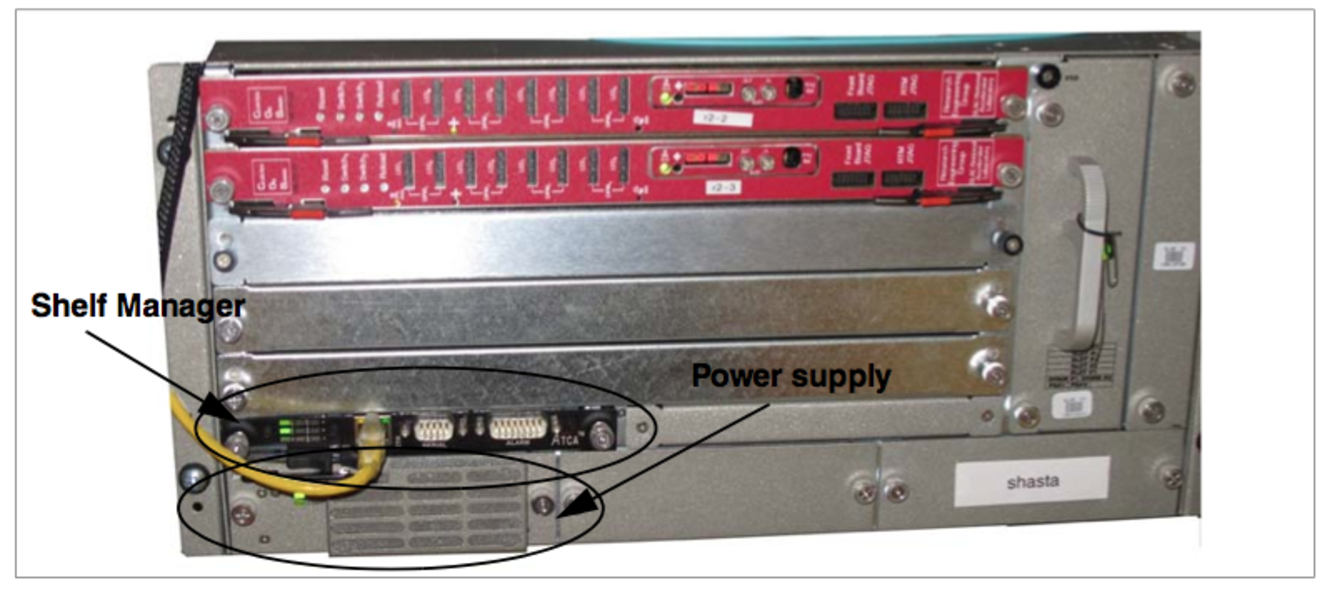
\includegraphics[scale=0.6]{shelf-front.pdf}
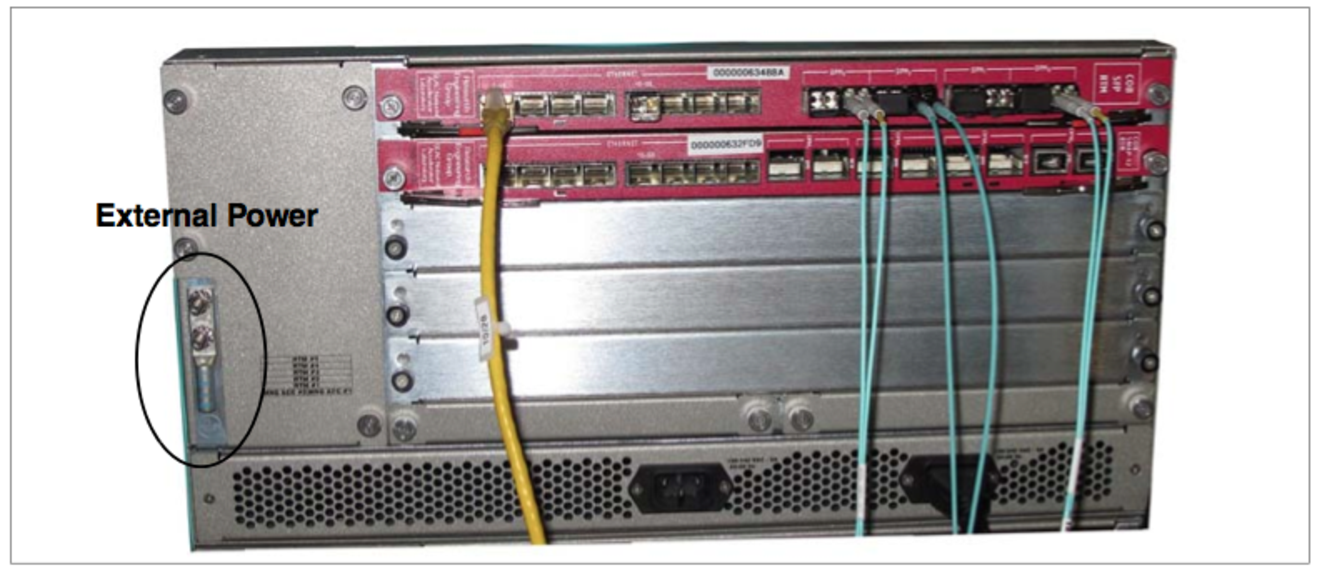
\includegraphics[scale=0.6]{shelf-back.pdf}
\caption{Front (top) and back (bottom) views of 5-slot ATCA shelf with two slots
occupied.}
\label{fig:frontShelf}
\end{figure} 

\subsubsection{The Front Board}
\label{sec:frontboard}
The Front Board constitutes the heart of the ATCA eco-system. 
From a shelf's perspective that board is simply a PCB board, 
8U wide x 280 mm deep and which plugs into one of its front slots. 
The board's rear side contains three logical Zones.
Zones 1 and 2 connect directly to a shelf's backplane. 
Zone 1 provides access to shelf power (+48 VDC) as well as the
I2C communication channels which the board uses to communicate with its shelf manager. 
Zone 2 provides access to the high-speed, differential pairs connecting boards together. 
The area encompassed by Zone 3 is application defined, but reserved for connections 
to the board's RTM.
A photograph of a representative Front-Board, 
showing connectivity to an RTM (using PICMG 3.8) 
is illustrated in Figure \ref{fig:frontBoard}.

The SLAC DAQ Toolkit includes an FB called the ``Cluster on Board'' (COB), which is
described in detail in Section \ref{sec:COB}.
This board is generic in that it is designed to be used in multiple experiments.
The external I/0 requirements of a given experiment can be satisfied by producing 
custom RTMs.


\begin{figure}[tbh]
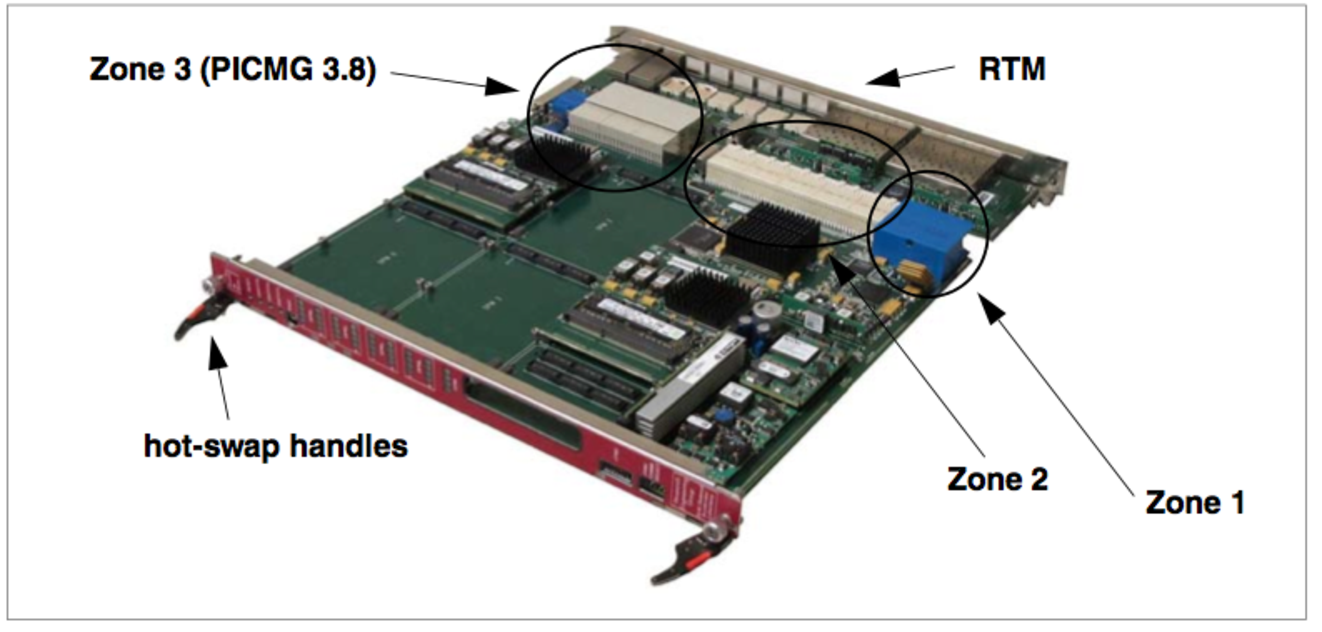
\includegraphics[scale=0.8]{front-boardpdf.pdf}
\caption{Representative ATCA front-board.}
\label{fig:frontBoard}
\end{figure} 

\subsubsection{Rear Transition Module}
\label{sec:rtm}
The RTM (Rear-Transition-Module) is simply a PCB board, 
8U wide x 70 mm deep which is used to house a Front Board's 
external I/O interface. 
The RTM connects to its front-board through Zone 3, which,
for the COB provides up to 120 differential pairs.
Each one of the COB's four Data Processor Module (DPM) bays 
is assigned 1/4 of those pins or thirty (30) pairs (see Section \ref{sec:COB}).
The specific I/0 requirements for different experiments (copper, fiber, custom 
connectors, etc.) can be satisfied with different RTM cards, which
plug into a generic COB board.
The RTM can thus 
be considered ``personality'' cards specific to a particular experiment. 


%\subsubsection{IPMI and Shelf Manager}
%\label{sec:shelfManager}
%ATCA adapts a somewhat locally autonomous philosophy with respect to environmental control and monitoring. As part of this model, each shelf has associated with it a single entity responsible for maintaining the health and safety of its infrastructure. That entity is called the Shelf Manager (ShMC). Front-Boards, through their own local controller (or IPMC) negotiate both individually and independently with their shelf manager for their own activation or deactivation. They do so by publishing changes to their state through dedicated I2C channels on the backplane.
%The shelf manager determines, based on hot-swap interface, when a board requires activation or deactivation. Power levels are negotiated based on both a board's request and the shelf's total available power. Shelf temperatures are maintained at safe levels autonomously by the shelf manager using information published by each board and adjusting power levels and fan-speeds accordingly.
%In short, once a shelf's power is applied and while its shelf manager is active, no external monitoring or control is necessary to maintain the shelf's health and safety.
%Although the health and safety of its shelf is maintained autonomously, the shelf manager still has provision for an external interface. Through this interface any information published to the shelf manager can be exported and the shelf manager can itself be configured. That physical interface is Ethernet and the shelf manager contains a TCP/IP Stack through which external communication is maintained. The logical interface for control and monitoring of the shelf is IPMI [18] and a wealth of tools exist, which interact with this interface.


\subsection{Cluster-on-Board}
\label{sec:COB}
The COB (Cluster-On-Board) is an ATCA compliant Front Board with a PICMG 3.8 Zone 3. 
Functionally, the COB serves as a carrier board for the Reconfigurable Cluster
Elements (RCEs) hosting the firmware and software developed for 
a given experiment (see Section \ref{sec:RCE}). 
Those RCEs are mounted on mezzanine boards 
%(see Section \ref{sec:Mezzanine}), 
which in turn plug into one of five bays on the COB. 
The bays are connected to the COB's two separate, 
independent Interconnects as well as its Zone 3 connectors. 
Interconnects provide arbitrary, high speed communication 
paths between the elements contained on the bay's mezzanine boards,
both (it is important to note), inter and intra COB.
Although rated up to 300 watts, when fully populated with five mezzanine boards, 
a COB draws closer to 120 watts. 
This board is one deliverable from SLAC's R \& D program on high-speed DAQ. 
As such, LBNE simply purchases this board and from its perspective, 
that board consequently requires neither design nor development.
A photograph of a COB (in preproduction form) with its five bays 
occupied is shown in Figure \ref{fig:cob}.


\begin{figure}[tbh]
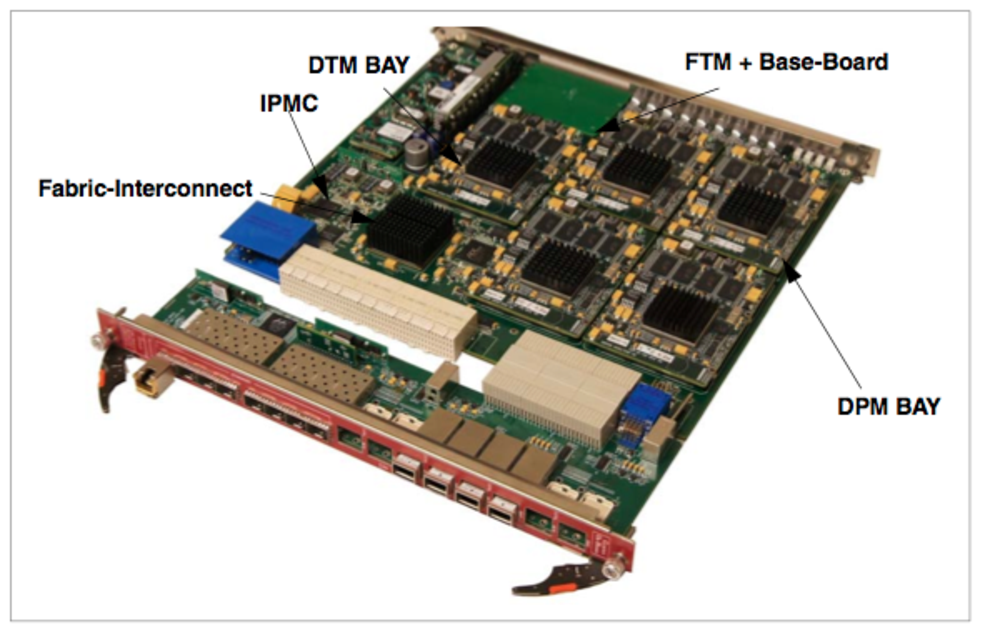
\includegraphics[scale=0.8]{cob-photo.pdf}
\caption{Pre-production COB.  }
\label{fig:cob}
\end{figure} 

The COB contains five (5) bays; one (1) Data Transport Module (DTM) bay 
and four (4) Data Processing Module (DPM) bays. 
Although all bays share identical form factors and connectors, 
they can be differentiated, primarily by how they connect to Zone 3,
with the DTM connecting only to its power connector and the DPM 
only to its signal connectors.

The mezzanine board plugged into the Data Transport Module (DTM) 
contains a single RCE that has the fixed, dedicated responsibility for 
managing both of the board's interconnects. 
For this purpose it contains specific firmware and software. 
For example, as one responsibility, it must maintain the 
configuration and supervise the 10G-Ethernet switch contained 
within the fabric interconnect. 
That switch's management interface is a single lane PCIe. 
To communicate with this switch, the RCE contains a 
PCIe Protocol-Plug-In (firmware, see Section \ref{sec:RCE}) 
as well as the tools (software) to configure and monitor that switch. 
Note, however, that while the DTM's RCE has predefined, base 
responsibilities it also remains accessible for user applications.

The mezzanine board plugged into a Data Processing Module (DPM)
bay contains two (2) RCEs. 
Each DPM provides connections to thirty 
(30) differential pairs originating from the RTM, 
but carried through the COB's Zone 3 signal connector. 
The mapping of those thirty pairs to the mezzanine board's 
two RCEs is arbitrary and determined by application. 

\subsection{Interconnects}
\label{sec:Interconnects}
There are two distinct ``interconnects''  providing communication 
between RCE's: the
``fabric'' interconnect and the ``base'' interconnect.


The fabric interconnect contains, as its principal feature, 
a local, 10-Gigabit Ethernet (10-GE).
Packets are switched on that network using a commercial ASIC
that is a fully compliant Layer-2, 10G-Ethernet switch. 
Although fully provisioned for buffered transfer, switch operation is, 
by default, cut-through with an ingress/egress latency of less than 200 Nanoseconds.
It is also a fully managed switch with a PCIe interface connected to the DTM's RCE. 
Through its interconnect the COB's RCEs appear as nodes on that Ethernet. 
The interconnect allows its physical network to be extended to both nodes 
and networks external to the COB. 
Those networks could be, for example, other COBs residing in the same shelf, 
or even nodes physically disjoint from both COB and its shelf.
%
%Internal to its shelf, the interconnect extends its network through its connections to Zone 2 of its backplane, specifically those connections to that backplane's fabric interface. The interconnect has individual connections to each of the thirteen slots of the shelf's backplane. With a full mesh backplane, this allows each network of every COB to be connected to each network of every other COB. External to its shelf the interconnect extends its network through its connections to the COB's fiber-optic transceiver bay. That bay can contain up to eight (8) SFP+ transceivers [20].
%The interconnect's switch is organized in units of Ports. Each port is composed of four lanes and each lane is constructed from two differential pairs. Each lane forms a full-duplex channel with one pair allocated for transmission and one pair for reception. Each lane of each port is capable of operating independently at a fixed set of speeds ranging from 1.0 Gigabits/second up to 12.5 Gigabits/second. Lanes may also be bound together to form a single Ethernet channel which operates at four times the speed of any one lane. For LBNE, which carries 10-GE, the switch is configured to run XAUI, requiring four lanes, each operating at 3.125 Gigabits/second. The switch contains twenty-four (24) ports. Those twenty-four ports are allocated to the fabric interconnect as follows:
%\begin{itemize}
%\item One (1) port connected to the DTM bay (one RCE).
%\item Eight (8) ports connected to the four DPM bays (two per bay, one for each RCE).
%\item Two (2) ports are connected to the SFP+ transceiver cage.
%\item Thirteen (13) ports are connected to the fabric interface (P2).
%\end{itemize}
%In short, within a shelf, the fabric interconnect allows for the formation of a uniform Ethernet populated with a flat space of RCE nodes.

The base interconnect's principal function is to manage 
and distribute synchronous timing to the COB's five bays.
Note that unlike the fabric interconnect the protocol 
distributed over this interconnect is application specific. 
%The distribution model for the base interconnect allows timing to originate from one of three potential sources:
%\begin{itemize}
%\item Internal, where the source is the base interface.
%\item External, where the source is the COB's Front-Transition-Module (FTM).
%\item Local, where the source is the COB's DTM.
%\end{itemize}
%Internal timing was described above. External timing allows the timing source to originate off the shelf. The FTM is a bay which contains an application %specific, small “PMC-like” daughter board. Logically, the FTM serves the same role on the front of the COB as the RTM does on its rear, that of media %adaptation. Eight (8) differential pairs from this daughter board connect directly to the base interconnect and eight (8) differential pairs connect to the %DTM's RCE. Those eight pairs are intended to allow that RCE supervision of the FTM. Local timing allows the board to operate either stand-alone or %perhaps more usefully provide a simulation of timing which would normally be sourced either internally or externally.
%LBNE has purpose built versions of both FTM and base board. Those version are described in Sections 2.6.5 and 2.6.6:


\subsection{Reconfigurable Cluster Element}
\label{sec:RCE}
The Reconfigurable Cluster Element (RCE) is a bundled set of hardware, 
firmware and software components. 
Together, those components form a generic computational element 
targeted to process efficiently, with low latency, those
kinds of data found passing through HEP DAQ systems. 
%The RCE is optimized for those three features. 
Physically, one element can be contained in a footprint of less than 32 cm$^2$, 
typically draws less than eight (8) watts, costs (in small quantities) 
around \$1000 and contains a native 10-Gigabit Ethernet interface. 
The combination of elements and switch define a Cluster and 
the nature of ethernet as well as functionality within that switch 
allows for the composition of arbitrary numbers of cluster hierarchies. 
For example, from the RCE perspective, the COB represents a single cluster 
of nine (9) RCEs and its ATCA shelf is simply a container for a 
single level hierarchy of up to fourteen (14) nine-node clusters. 
A block diagram of the major physical features of the RCE is illustrated in Figure 
\ref{fig:RCEblock}.

\begin{figure}[tbh]
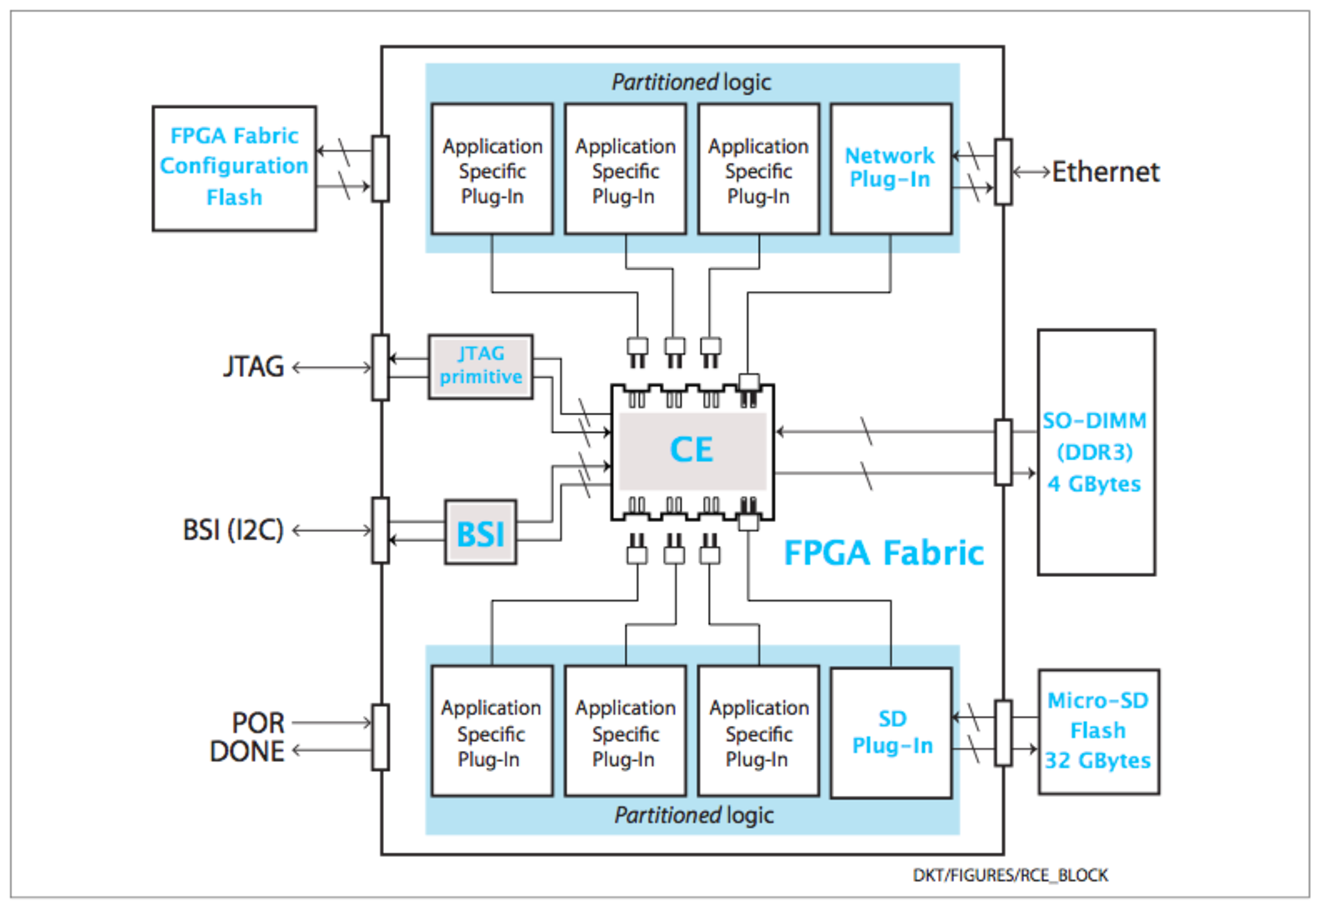
\includegraphics[scale=0.8]{rce-block.pdf}
\caption{Block diagram of the RCE.}
\label{fig:RCEblock}
\end{figure} 

The principal implementation feature of the RCE is its reuse 
of System-On-Chip (SOC) technology, specifically, members of 
Xilinx Virtex family.
The current generation of RCE, which we propose to use
for the 35t protoype uses a Zynq chip, which is part of the Virtex-7 family. 
The RCE is neither processor, FPGA or DSP. 
Instead, it can be simultaneously any combination of the three. 
Within its fabric, the FPGA contains both soft (user defined) 
and hardened (manufacture defined) silicon. 
That fabric is configured automatically on POR (Power-On-Reset) 
and is either downloaded directly from images previously stored on the 
FPGA's configuration (platform) flash, or indirectly through the RCE's JTAG interface.
Note also that the platform flash is itself programmed through the RCE's 
JTAG interface. 
The RCE employs standard Xilinx tools and software to program the FPGA.
Xilinx refers generically to its set of different, hardened silicon as resources. 
Among the more important of those resources are high speed serializers/deserializers,
 I/O adapters, DSP tiles, dual-port RAM and of course, its processor. 
The RCE allocates the processor as well as a modest number of additional
 resources and soft silicon for its Cluster Element(CE). 
The CE has exclusive use of, but interfaces indirectly with its external
DDR3 memory and micro-SD flash system. 
Memory is packaged as SO-DIMM and the micro-SD flash is removable, 
allowing its capacity to be determined by user application.

The core of the CE is a processor that in the Gen 3 RCE is an ARM processor running Linux. 
This will greatly facilitate software development.


%The BSI‘s (Boot-Strap-Interface) principal function is to reset the CE. However, it also contains the initial configuration information necessary for the CE's bootstrap loader to boot its processor. The BSI is outside the CE so that its configuration may be retained over resets of the CE. External to the FPGA the BSI appears as a standard I2C device and receives its command and control through that interface. Note, for the COB, that device is controlled and monitored through its IPMC.

%To provide isolation between system and user firmware and insure reproducible behavior, system firmware is partitioned [53] away from application specific logic. System firmware is defined as the CE, the BSI, JTAG support and both Network and SD Plug-Ins.
%The CE, which is both at the heart of the entire RCE and contains a significant fraction of the user's intellectual investment is described in Section \ref{sec:CE}. The remainder of the fabric, both hardened and soft silicon is reserved for application specific logic. That logic and its relationship with the CE is described below.

%Although both user defined and implemented, any application specific logic, does of course require information exchange between it and its CE1. The interface model which allows such exchanges is the plug and socket. To follow that model, the user wraps their implementation specific logic with a thin veneer of system provided firmware. That wrapper is the plug and the combination of user logic and its plug is called a Protocol-Plug-In or PPI. When wrapped, that logic is now capable of being plugged into any of the eight predefined sockets on the CE. And once plugged in, both PPI and CE are now able to exchange information.

%Although bundled with its base system the RCE itself takes advantage of this model to “glue” its Ethernet and SD interfaces to the CE. Both are good examples of one class of PPIs which must interface outside their FPGA.  Such PPIs when plugged into their CE have as their closest analogy the classic I/O device and processor model. However, unlike that model the PPI model coupled with the resources offered by the FPGA fabric provides an essentially unlimited way to either customize or mold the CE to arbitrary devices and protocols. Of course, the user is not limited to using the fabric and its resources solely for I/O. One can define PPI whose sole purpose is to take advantage of the DSP tiles and combinatoric logic of the FPGA to process rather than transfer data. LBNE can use this functionality to its advantage in performing its feature extraction.


\subsubsection{Software Services}
\label{sec:Services}
The RCE includes bundled software to accelerate and leverage 
the development of application specific code for the CE. 
Some set of this software is linked to and executes with those 
applications (system resident software), while a subset is in the 
form of tools that operate cross-platform. 
Any and all system resident software is distributed with each RCE 
and if used, is dynamically linked to its corresponding applications. 
Remote tools and any software updates have a well defined release and
distribution mechanism. 
JIRA is used for a bug-tracking and reporting system. 
Here is a summary of the software services bundled with the RCE:
\begin{itemize}
\item Bootstrapping: A generic bootstrap loader which allows, on reset,
transfer to arbitrary code based on an externally controlled configuration 
parameter called its current vector (contained within the BSI). 
The code loaded and executed by the loader is assumed stored in the RCE's 
micro-SD device. The code pointed to by any specific vector is called a bootstrap. 
Bootstraps may be either standalone code or
code which loads and transfers control to other code (a secondary loader). 
The CE may contain and transfer control to an arbitrary number of different 
bootstraps. 
For LBNE, on reset, control is transferred to a secondary bootstrap 
which starts up Linux (see below).
\item Operating/System: 
Although the CE is itself O/S agnostic, its system resident software is 
not and depends on functionality best provided by the services of an underlying O/S.
In the Gen 3 RCE, this will be Linux.
\item Persistency:
Access to micro-SD based media using its bundled Protocol
Plug-In (PPI). 
That media is formatted as FAT-16 and is used by the CE 
for storage of system code and configuration (see bootstrapping above). 
However, that media is available directly to applications 
for storage of their own application specific code and configuration.
\item Networking: Includes a complete TCP/IP stack. 
The stack's MAC layer is satisfied by the RCE's bundled 10G-Ethernet PPI. 
The user interfaces to that stack are POSIX compliant.
\item Linking: The same dynamic linker used to bridge system and user code.
\item PPI support: Interrupt and reset support for an application's PPI.
\item Debugging: Support for both local and remote debugging. 
Local debugging (SMD) interfaces to JTAG through standard Xilinx tools. 
Remote, network based, debugging uses the GNU interface.
\item Diagnostics: Built-in self-tests as well as diagnostics. 
These are included on the CE as an alternate boot image providing the 
ability to rescue or repair inadvertent burns of the micro-SD media.  
Development employs the GNU cross-development environment.
\end{itemize}

%\subsubsection{Mezzanine Board}
%label{sec:Mezzanine}
%The mezzanine board is one physical implementation of the abstract RCE described above in Section \ref{sec:RCE}. It is a PCB board (100 mm x 80 mm) which hosts either one or two elements of RCE. A mezzanine board plugs into any one of the five bays contained on a COB.
%Power (+6 VDC) to this board is applied using two separate, but identical connectors. One connector is assigned to each element of the board. Those connectors provide, in addition to power, a presence sense pin as well as an enable pin for that power. The board's two, internal PDS (Power-Distribution-Systems) takes that input voltage, divides it down and distributes the necessary, well regulated voltages to each element. Each PDS can source 25 Watts.

%A high-speed, high density, differential connector carries signals between the COB and the elements of the mezzanine board. Those signals include:
%\begin{itemize}
%\item  To and from RTM (thirty pairs).
%\item To and from the Fabric interconnect (sixteen pairs).
%\item To and from the Base interconnects (eight pairs).
%\item JTAG.
%\item To and from the IPMC (I2C); one per element.
%\end{itemize}
%On each of its two I2C channels the board contains, in addition to the element's BSI  various I2C devices which provide %the following information:
%\begin{itemize}
%\item PDS status.
%\item Board and die temperatures.
%\item Element serial number (64 bit).
%\item Persistent, configuration information (MAC addresses, element wiring, etc.)
%\end{itemize}

%The COB's IPMC uses that information to “plug and play” with its bays, including their activation as well as in the monitoring of their health and safety.
%To illustrate both mezzanine concept and its relationship to the RCE, a photograph of the prototype (single element) GEN-II RCE, mounted in a mezzanine board is shown in Figure \ref{fig:mezz}.

%\begin{figure}[tbh]
%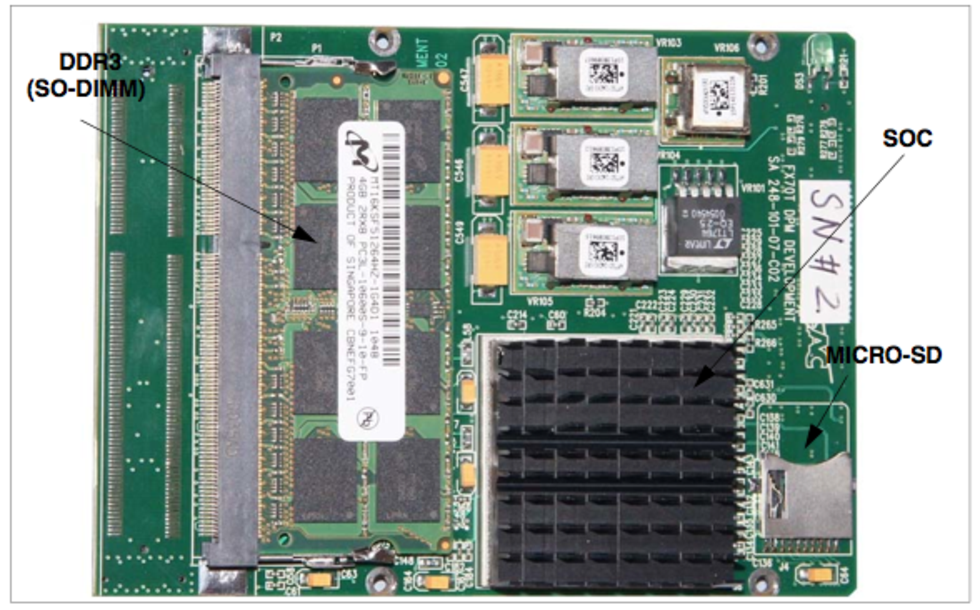
\includegraphics[scale=0.8]{mezzanine.pdf}
%\caption{A single element RCE on a mezzanine board.}
%\label{fig:mezz}
%\end{figure} 


%\subsubsection{Pretty Good Protocol}
%\label{sec:PGP}
%The Pretty Good Protocol (PGP)\cite{bib:pgp} is a 
%VHDL module which facilitates the bi-directional transmission 
%of frame based messages over a two-wire physical link.  
%PGP is openly and freely available and can be deployed on any 8B/10B SerDes link, be it copper or optical, with low overhead (96\% efficient after 8B/10B conversion).   The protocol allows for unlimited frame size based on 512byte cells; large frames are broken down into these cells for more efficient transport.  

%Each physical PGP link (lane) contains 4 virtual channels, each with a separate firmware interface.  In addition, each virtual channel on a lane can be either an upstream or downstream link (even at differing line rates).  Lanes can also be "bonded" together for a wider data path; for instance four 3.125 Gbps lanes can be bonded to create what (functionally and transparently) is a single 12.5 Gbps lane.   

%Many tools exist for implementing and handling PGP data for the RCE-based system and it  would be beneficial, although not strictly necessary, to use this protocol if the RCE-based DAQ is implemented.  
